\documentclass{article}
\usepackage[utf8]{inputenc}
\usepackage{graphicx} 
\usepackage{hyperref}
\title{Stock}
\date{March 2014}

\begin{document}
We today focus on a stock named ZYXH, while this analysis procedure might suit for many other different cases.
\section{Fundamental Analysis}
\subsection{Economical Analysis}
Since GDP of China always be stable, another aspects may account more.

Though Central Bank and Four major commercial banks of China are cooperating in depressing so called Yu'ebao, that actually in my opinion stablized the financial world because this industry used to be totally controled by the former, while Yu'ebao made the interest rate market became volatile. 

No matter whether the traditional banks or Yu'ebao can win the game, here must be an overall revolution in financial market both fundamentally and structurely. Thus one cannot ignore this potential challenge in the future to any extent if he invests stocks.

Another essential economical affair occurred recently is related to Central Bank too. The exchange rate, i.e. the value of China Yuan in global market is down rapidly after a continuous increase in past few years which makes ex-rate escalate to like 6:1. The latest quote of China yuan to US dollar is about 6.2128. This can be a very serious problem for export oriented firms.

\subsection{Industry Analysis}
\subsubsection{outlook of industry}

For ZYXH, it belongs to Industry of Medicine. 

Not exaggerating, Medicine is one of the few strong industries in such downturn stock market. By an article published March 27th, Medicine index rises 4.18\%, and the Medical Service board makes the most contribution which rises 26.92\%.

There are several reasons of policy of course. The 18th National People's Congress released several revolution blueprints over Medicine (Health care reform) to alleviate conflicts between hospitals and patients. For some more information, please visit: \url{http://www.dwz.cn/fA93j}

Since the Health Care Reform could have a long way to go, we can predict that the benefit to Medicine industry will be constant in the foreseeable futrue. 

\subsubsection{Competitions inside industry}
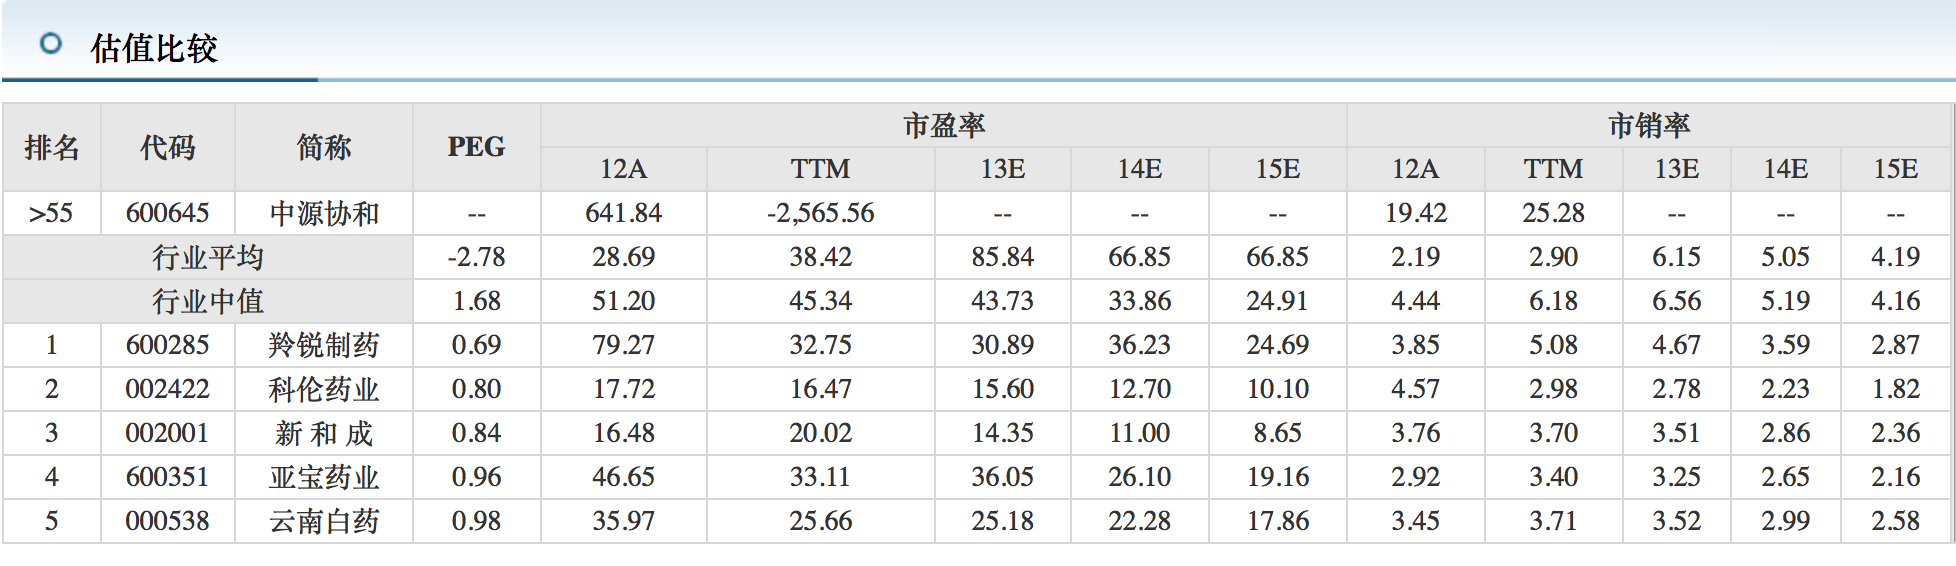
\includegraphics[width=5in]{value_compare} 
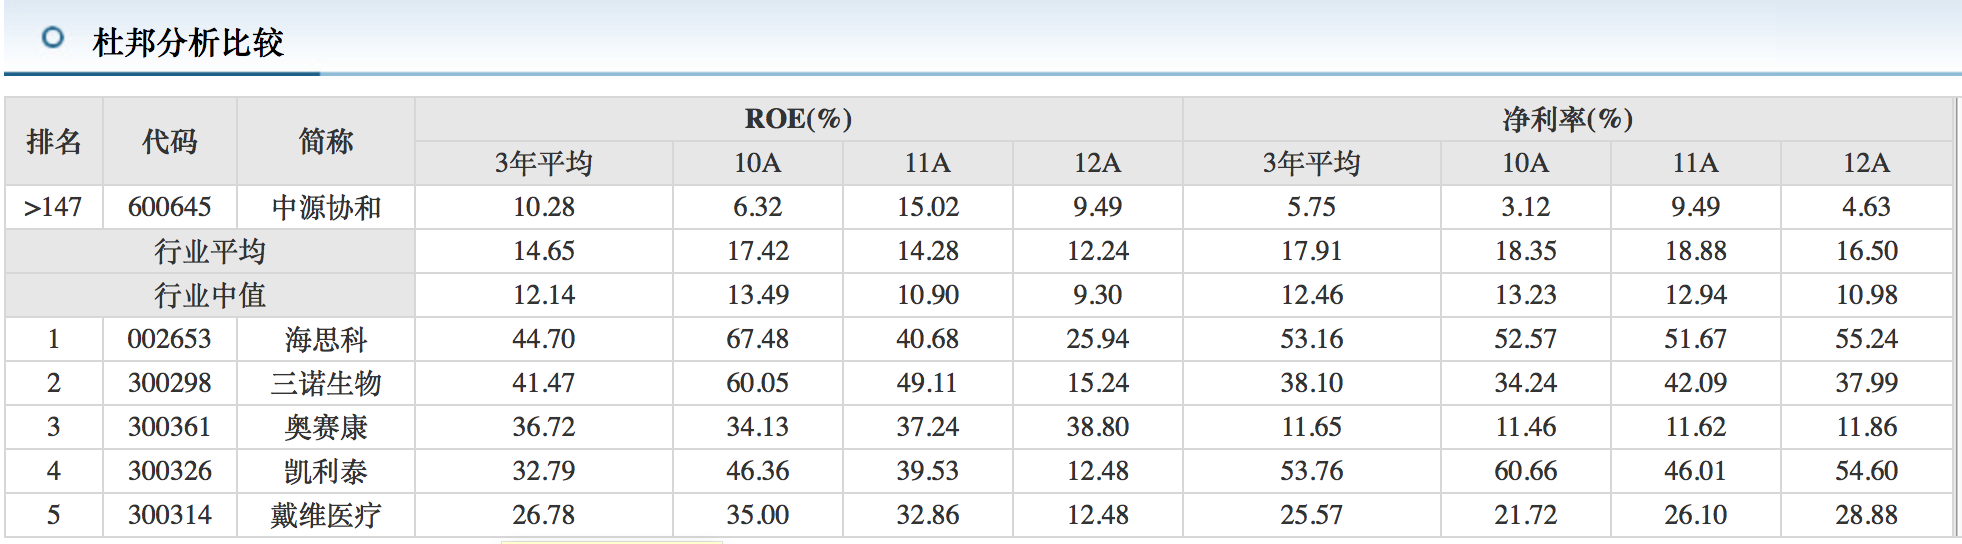
\includegraphics[width=5in]{dubang} 

From the above tables we can clearly see that ZYXH perform really bad compared with its competitors. Especially the P/E ratio is tens of times over other competiters, which means this stock is nothing but bubble.
In this sense, by no means I will buy this stock. But wait, for speculators, this is somewhat a better security than other relatively stable stocks.

Speaking of which, this industry is seriously dependent on patents. And technology improvements can save a struggling company from bankrupcy and to be outstanding overnight. Reversely, if one firm can't go on in researching then it may soon be eliminated by the market.

\subsection{Fundamental Analysis}
Below is the financial report of ZYXH over seasons.\\
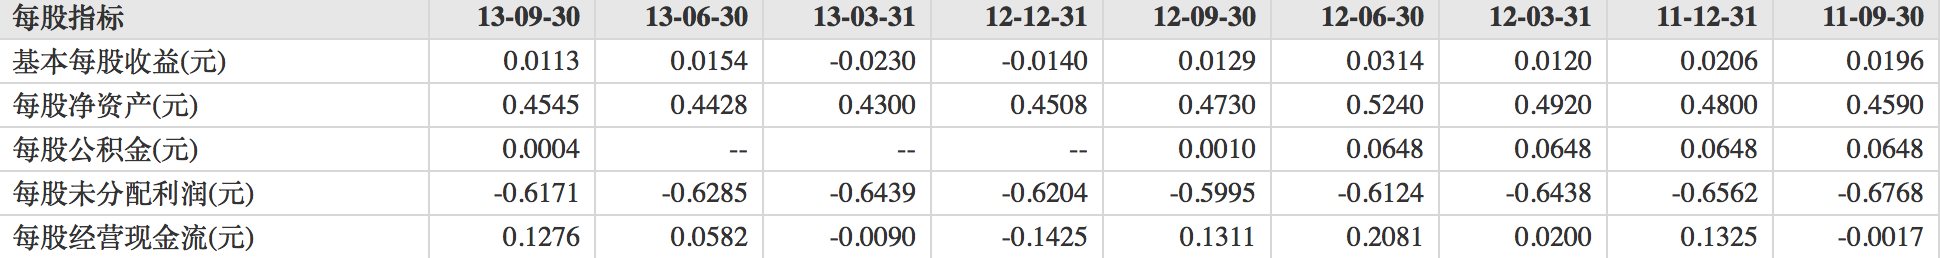
\includegraphics[width=5in]{report1} 
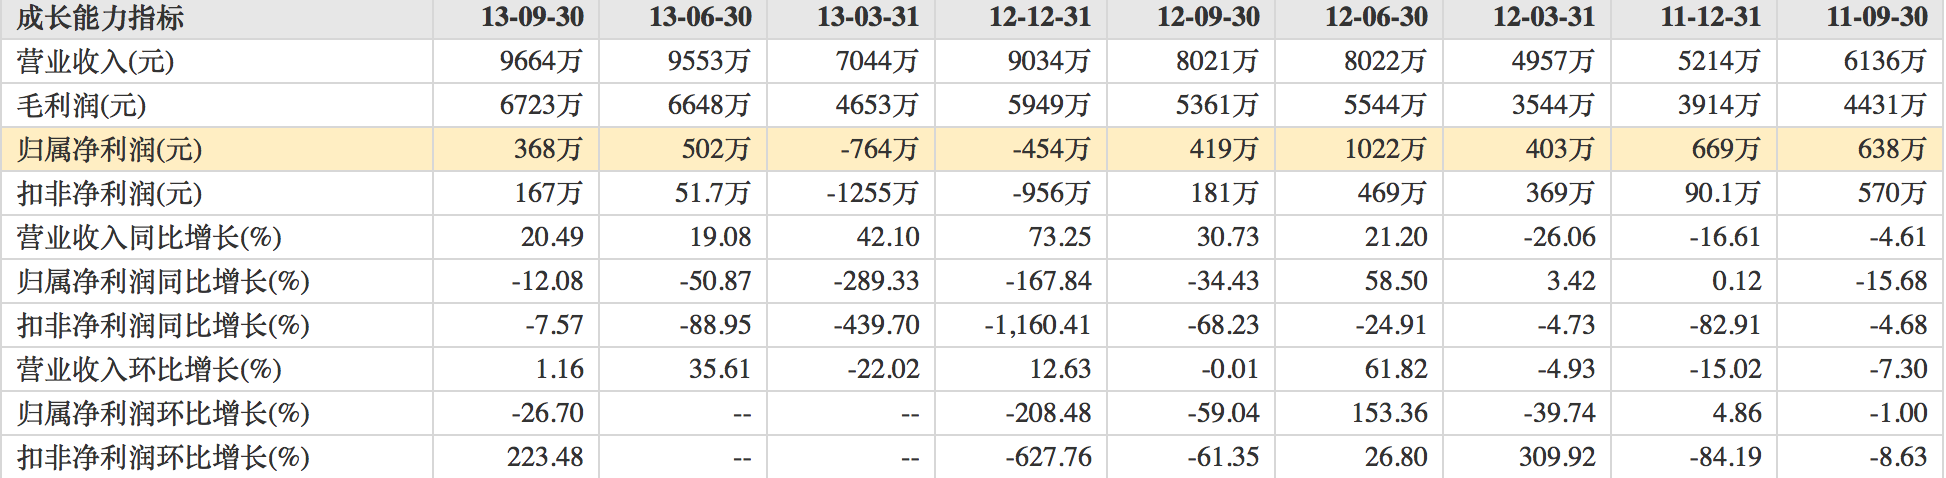
\includegraphics[width=5in]{report2} 
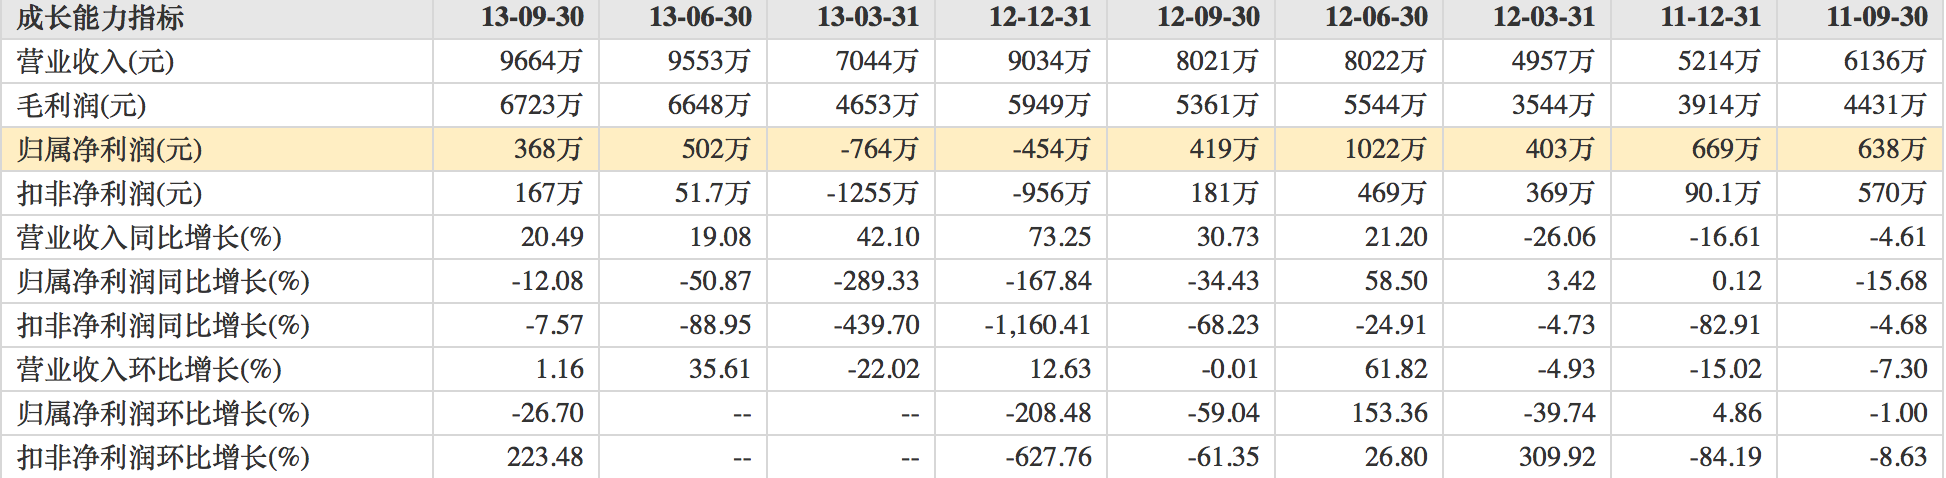
\includegraphics[width=5in]{report2}

As we can see, though didn't deficit recently, nearly zero earnings been made per share, far less than what other con-industrial firms made. And it is that no signal of improvement that makes the situation even worse.

A serious problem seems suffering a currency shortage.\\
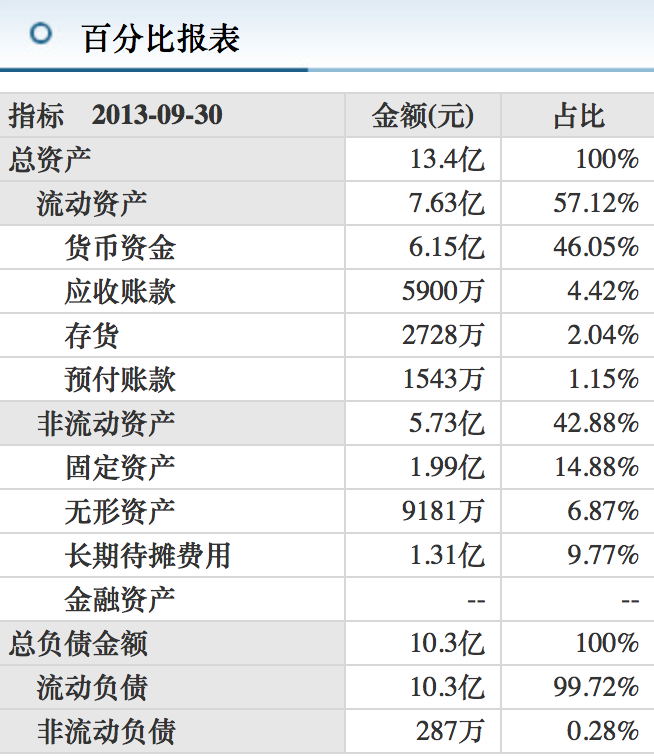
\includegraphics[width=2in]{percent}

Notice that current liabilities is larger than current assets. Which means 
\[
    Current Ratio = \frac{CurrentAssets}{CurrentLiabilities} < 1
\]
Regularly, this ratio should be approximately 2 if a firm perform well. The lower the ratio, the more serious the liability problem the firm has. This is a intensive signal tell us that 'this is a trash security'.

Also, the Net Working Capital is actually negative, bad situation.

Let's talk about Inventory Turnover
\[
    Inventory Turnover = \frac{Annual sales}{Inventory} = 0.566
\]
Intuitively, this ratio must be close to 1. Again this seems not good. And consequently the large inventory unsold could result in a consecutive liability problems mentioned above.

Needless to say, the Net Profit Margin is also of tragedy. Now let's finally talk about Price-to-Book Ratio:
First
\[
    Book Value = \frac{Equity}{Number of shares} = 3.1\times 10^8 / 34929 \times 10^4 =0.8875 
\]
Then
\[
    P/B = \frac{stock price}{book value} = 25.54/0.8875=28.777
\]
Now with this obvious result one can claim that ZYXH is nothing but a bubble. 





\end{document}
